\documentclass{hw}
\usepackage{amsmath,amssymb}
\usepackage{graphicx}
\usepackage{caption}
\usepackage{subcaption}

\title{Threshold Phenomenon in a Nonlinear Heat Equation}
\author{}
\date{}

\begin{document}
\maketitle
\section{Introduction}

This paper concerns the behavior of the following non-linear heat equation given by
\begin{gather}
u_{t}=u_{xx}+u^{3},\ 0<x<\pi,\ t>0\\
u(0,t)=u(\pi,t)=0,\ t>0\\
u(x,0)=u_{0}(x),\ 0<x<\pi.
\end{gather}

This system corresponds to several physical situation, including exothermic reactions between
chemicals. We know that this equation has a solution $u(x,t)$, but it may help us to consider the
\textit{steady state} equation corresponding to this system. The steady state arises from holding
time constant; thus, our differential equation becomes dependent only on $x$.

\section{Steady State Analysis}
The steady state equation of $(1)$ is given by
\begin{gather}
u_{xx}+u^{3}=0\\
u(0)=u(\pi)=0.
\end{gather}
We want to find a solution $u_{s}(x)$ that satisfies the following properties
\begin{enumerate}
\item If $u_{0}(x)<u_{s}(x)$, then $u(x,t)\to u_{s}(x)$ as $t\to\infty$.
\[
\lim_{t\to \infty}u(x,t)=u_{s}(x).
\]
In this case, the solution to $(1)$ would independent of time. If this property is fulfilled, then
there is a \textit{global solution} $u(x,t)$ to the boundary value problem described in $(1)$.
\item If $u_{0}(x)>u_{s}(x)$, then $u(x,t)$ blows up in a finite time. This means that the solution
tends towards infinity in a finite time $T$.
\[
\lim_{t\to T}u(x,t)=\infty.
\]
This case if often indicative of a singularity in the solution $u(x,t)$. The solution $u$ of $(1)$
would not be global in this case.
\end{enumerate}
We can now attempt to solve this steady state problem.

\subsection{Solution to the Steady State Problem}
We are attempting to solve the ordinary differential equation
\[
u''=-u^{3}.
\]
Multiplying both sides of the equation gives us
\begin{align*}
u''u'&=-u'u^{3}\\
\int u''u'&=\int -u'u^{3}\\
{1\over2}(u')^{2}&= -{1\over4}u^{4}+c\\
2(u')^{2}&=-u^{4}+c_{1}.
\end{align*}
This first order equation does not lend itself to separation of variables as readily as we would like
(although it is possible if we want to deal with imaginary numbers). Instead, we will use a technique
called the \textit{shooting method} in order to determine a solution. The shooting method provides
us with a way to relax boundary conditions into initial conditions. Recall that $(5)$ provides us
with boundary conditions that arose from the steady state of $(1)$. We will leave the first boundary
condition alone and change the second boundary condition so that $2u'(0)^{2}=a^{4}$. This will allow
us to factor the resulting term:
\begin{align*}
u'(x)^2&={1\over2}(a^{4}-u^{4})\\
{\du\over\dx}&= \sqrt{{1\over2}(a^{2}+u^{2})(a^{2}-u^{2})}\\
{\dx\over\du}&= {1\over\sqrt{{1\over2}(a^{2}+u^{2})(a^{2}-u^{2})}}.
\end{align*}
Integrating both sides and substituting $s$ for $u$ gives us
\[x=\int_{0}^{u}{1\over\sqrt{{1\over2}(a^{2}+s^{2})(a^{2}-s^{2})}}\mathop{ds}.\]
We can now make another substitution for $s$ in terms of $t$. Letting
\[
s=\sqrt{{a^2t^2\over2(1-t^2/2)}}
\]
yields
\[
a^2+s^2={2a^2\over2(1-t^2/2)}\qquad\qquad\text{and}\qquad\qquad
a^2-s^2={a^2(1-t^2)\over(1-t^2/2)}.
\]
We also have
\[
\mathop{ds}={a(t-1)(t-2)\over2\sqrt{2}(1-t^2/2)^{3/2}}\dt,
\]
which gives us the new integral
\[
ax=\int_{0}^{\sqrt{\frac{\displaystyle2u}{\displaystyle a^2+u^2}}}{1\over\sqrt{(1-t^2)(1-t^2)}}.
\]
We may notice that this integral is one of the ways to define $sn(x,k)$. Rewriting it in terms
of our Jacobi elliptic function gives us
\[
x=\int_{0}^{sn(x,k)}{1\over\sqrt{(1-t^2)(1-t^2/2)}}.
\]
%% TODO -- Expand on this information
Finally, we have a solution $u(x)$
\[
u(x)={a\ sn(ax,\sqrt{1/2})\over\sqrt{2-sn^{2}(ax,\sqrt{1/2})}}.
\]
Recall that the first positive zero of $sn(x,k)$ is given by
\[
K=\int_{0}^{1}{1\over\sqrt{(1-t^2)(1-{t^2\over2})}}\dt.
\]
Then $u(x)=u_{s}(x)$ provided that $a=2K/\pi$. We can see the results via these Mathematica plots:
\begin{figure}[h]
\centering
\begin{subfigure}{0.45\textwidth}
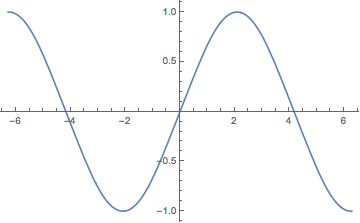
\includegraphics[scale=0.5]{u_of_1_x}
\end{subfigure}
\hfill
\begin{subfigure}{0.45\textwidth}
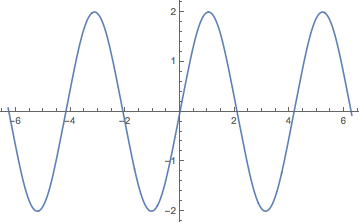
\includegraphics[scale=0.5]{u_of_2_x}
\end{subfigure}
\caption{The graphs of $u_{s}(x)$ for $a=1$ and $a=2$}
\end{figure}

\noindent It appears that, for $a=1$, $u_{s}(x)$ behaves similar to $\sin{x}$.

\begin{figure}[h]
\centering
\begin{subfigure}{0.45\textwidth}
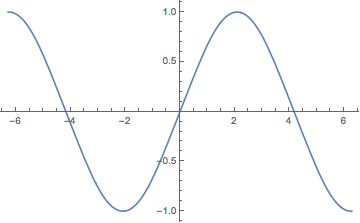
\includegraphics[scale=0.5]{u_of_1_x}
\end{subfigure}
\hfill
\begin{subfigure}{0.45\textwidth}
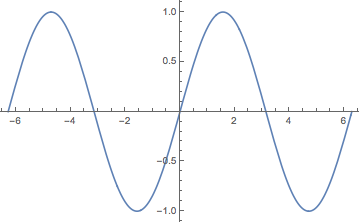
\includegraphics[scale=0.5]{sinx}
\end{subfigure}
\caption{The graphs of $u_{s}(x)$ for $a=1$ and $\sin{x}$}
\end{figure}

\subsection{Average of the Steady State Solution}

If we can find the average temperature of the steady state, then we know that our function $u(x)$
has a global solution (otherwise there would be points in the range of $u$ for which $u$ blows up).
We will want to show that
\[
{1\over\pi}\int_{0}^{\pi}u(x)\dx={\sqrt{2}\over2}.
\]
To begin, let
\[
y=\int_{0}^{x}u(t)\dt
\]
and $v(y)=u^{2}(x)$ where $x=x(y)=y^{-1}(x)$. 

\end{document}
